\documentclass{../mynotes}
%\usepackage[utf8]{inputenc}
\usepackage[margin=1in]{geometry}
\usepackage[usenames, dvipsnames]{xcolor}
\usepackage{graphicx}
\usepackage{mathtools}
\usepackage{amssymb}
\usepackage{amsthm}
\usepackage{fancyhdr}
\usepackage{adforn}
\usepackage{xparse}
\usepackage{tikz}
\usetikzlibrary{fadings}
%\usetikzlibrary{matrix, positioning, calc}
% Additional math macros that I want in both my notes and my psets
\usepackage[sc, noBBpl]{mathpazo}
\usepackage{mathrsfs}
\usepackage[T1]{fontenc}
\usepackage{calligra}
\usepackage{microtype}
\usepackage[all]{xy}
\usepackage{slashed}
\newcommand{\A}{\mathbb A}
\newcommand{\cat}{\mathsf}
\newcommand{\sC}{\cat C}
\newcommand{\sD}{\cat D}
\newcommand{\sS}{\cat S}
\newcommand{\sA}{\mathscr A}
\newcommand{\sF}{\mathscr F}
\newcommand{\sG}{\mathscr G}
\renewcommand{\P}{\mathbb P}
%\newcommand{\cO}{\mathscr O}
\newcommand{\cO}{\mathcal O}
\newcommand{\sI}{\mathscr I}
\DeclareMathOperator{\coker}{coker}
\renewcommand{\Im}{\operatorname{Im}}
\newcommand{\pt}{\mathrm{pt}}
\DeclareMathOperator{\Hom}{Hom}
\newcommand{\op}{^{\mathsf{op}}}
\newcommand{\Id}{\mathrm{Id}}
\DeclareMathOperator{\Mat}{Mat}
\newcommand{\m}{\mathfrak m}
%\newcommand{\p}{\mathfrak p}
\newcommand{\q}{\mathfrak q}
\newcommand{\pre}{\sC^{\text{pre}}}
\newcommand{\sh}{_{\text{sh}}}
\newcommand{\G}{\mathbb G}
\DeclareMathOperator{\Proj}{Proj}
\newcommand{\sM}{\mathscr M}
\newcommand{\sV}{\mathscr V}
\newcommand{\fU}{\mathfrak U}
\newcommand{\GL}{\mathrm{GL}}
\DeclareMathOperator{\Sym}{Sym}
% http://tex.stackexchange.com/questions/141434/how-to-type-sheaf-hom
\DeclareMathOperator{\shom}{\mathscr{H}\text{\kern -4pt {\calligra\large om}}\,}
\newcommand{\sL}{\mathscr L}
\DeclareMathOperator{\QC}{QC}
\DeclareMathOperator{\Supp}{Supp}
\newcommand{\sN}{\mathscr N}
\DeclareMathOperator{\Ann}{Ann}
\DeclareMathOperator{\Der}{Der}
\newcommand{\ctcpx}[1]{(#1)^{\text{der}}}
\newcommand{\Dist}{\mathsf{Dist}}
\newcommand{\shdi}{\operatorname{Sh}_{\Dist}}
\DeclareMathOperator{\Sh}{Sh}
\newcommand{\shz}{\mathsf{Sh}_{\text{\rm Zar}}}
\DeclareMathOperator{\Gr}{Gr}
% Source: http://tug.org/pipermail/xy-pic/2001-July/000015.html
\newcommand{\pullbackcorner}[1][dr]{\save*!/#1+1.2pc/#1:(1,-1)@^{|-}\restore}
\newcommand{\pushoutcorner}[1][dr]{\save*!/#1-1.2pc/#1:(-1,1)@^{|-}\restore}
\newcommand{\TDel}{\mathrm{2\Delta}}
\DeclareMathOperator{\Bl}{B\ell}
\newcommand{\cR}{\mathcal R}
\newcommand{\cL}{\mathcal L}
\newcommand{\cN}{\mathcal N}
\newcommand{\cH}{\mathcal H}
\newcommand{\cJ}{\mathcal J}
\newcommand{\cQ}{\mathcal Q}
\newcommand{\cZ}{\mathcal Z}
\newcommand{\cT}{\mathcal T}
\newcommand{\refR}{\reflectbox{\(\cR\)}}
\DeclareMathOperator{\ad}{ad}
\DeclareMathOperator{\Tr}{Tr}
\DeclareMathOperator{\tr}{tr}

\renewcommand{\a}{\alpha}
\renewcommand{\b}{\beta}
\newcommand{\e}{\varepsilon}
%\newcommand{\e}{\epsilon}
\renewcommand{\l}{\lambda}
\renewcommand{\L}{\Lambda}
\newcommand{\g}{\gamma}
\newcommand{\s}{\sigma}
\newcommand{\z}{\zeta}
\newcommand{\II}{\mathbb{I}}
\newcommand{\RR}{\mathbb{R}}
\newcommand{\NN}{\mathbb{N}}
\newcommand{\QQ}{\mathbb{Q}}
\newcommand{\ZZ}{\mathbb{Z}}
\newcommand{\CC}{\mathbb{C}}
\newcommand{\cB}{\mathcal{B}}
\newcommand{\cC}{\mathcal{C}}
\newcommand{\cD}{\mathcal{D}}
\newcommand{\cM}{\mathcal{M}}
\newcommand{\f}{\frac}
\newcommand{\p}{\partial}
%\renewcommand{\P}[3][]{\f{\partial^{#1} #2}{\partial #3 ^{#1}}}
\renewcommand{\P}[2]{\frac{\partial #1}{\partial #2}}
%\newcommand{\avg}[1]{\langle #1 \rangle}
\newcommand{\avg}[1]{\left< #1 \right>}
\newcommand{\?}{\overset{?}{=}}
\newcommand{\Int}{\int_{-\infty}^\infty}
%\newcommand{\ket}[1]{\left| #1 \right>} % for Dirac bras
%\newcommand{\bra}[1]{\left< #1 \right|} % for Dirac kets
%\newcommand{\braket}[2]{\left< #1 \vphantom{#2} \right|
% \left. #2 \vphantom{#1} \right>} % for Dirac brackets
\DeclarePairedDelimiter\bra{\langle}{\rvert}
\DeclarePairedDelimiter\ket{\lvert}{\rangle}
\DeclarePairedDelimiterX\braket[2]{\langle}{\rangle}{#1 \delimsize\vert #2}
\newcommand{\kb}[2]{\left\lvert #1 \middle\rangle\!\middle\langle #2 \right\rvert}
\newcommand{\dyad}[1]{\left\lvert{#1}\middle\rangle\!\middle\langle{#1}\right\rvert}%{\left| #1 \right>\left< #1 \right|}
\DeclarePairedDelimiter{\ceil}{\lceil}{\rceil}
\newcommand{\ul}[1]{\underline{#1}}
\def\normord#1{\mathop{:}\nolimits\!#1\!\mathop{:}\nolimits}
%\newcommand{\normord}[1]{{:}\!\mathrel{#1}\!{:}}

%vector calculus
\newcommand{\grad}[1]{\gv{\nabla} #1} % for gradient
\let\divsymb=\div % rename builtin command \div to \divsymb
\renewcommand{\div}[1]{\gv{\nabla} \cdot #1} % for divergence
\newcommand{\curl}[1]{\gv{\nabla} \times #1} % for curl

%lists are (a) (b) (c) by default
\renewcommand{\labelenumi}{(\alph{enumi})}

\newcommand{\term}{\emph}

%vectors
\renewcommand{\vec}[1]{\boldsymbol{\mathbf{#1}}}
\let\vaccent=\v % rename builtin command \v{} to \vaccent{}
\renewcommand{\v}[1]{\ensuremath{\mathbf{#1}}}
\newcommand{\uv}[1]{\ensuremath{\mathbf{\hat{#1}}}} % for unit vector
\newcommand{\gv}[1]{\ensuremath{\mbox{\boldmath$ #1 $}}} 
% for vectors of Greek letters

%\usepackage[framemethod=TikZ]{mdframed}
%\newenvironment{framedefn}[2][]{
%    \stepcounter{equation}
%    \begin{mdframed}[frametitle={Definition}]\relax%
%    \label{#2}
%}{\end{mdframed}}
\usepackage{hyperref}
\usepackage{siunitx}

%\usepackage[compat=1.1.0]{tikz-feynman}

% TODO fiddle with colors
\definecolor{newblue}{HTML}{1F98A6}
\definecolor{newred}{HTML}{D95448}
\definecolor{neworange}{HTML}{F29441}
\hypersetup{
	colorlinks,
	linkcolor=newred,
	citecolor=neworange,
	urlcolor=newblue!80!black,
}
\usepackage[all]{hypcap}
\pagestyle{plain}
\setcounter{tocdepth}{1}


\usepackage{titlesec}
\titleformat{\section}[frame]
  {\normalfont}
  {\filright
   \footnotesize
   \enspace Lecture \arabic{section}.\enspace}
  {8pt}
  {\Large\bfseries\filcenter}
\usepackage[dotinlabels]{titletoc}
\titlecontents{section}[1.5em]{}{\contentslabel{2.3em}}{\hspace*{-2.3em}}{\hfill\contentspage}

\renewcommand{\sectionmark}[1]{\markleft\thesection. #1}

\fancyhf{}
\fancyhead[RO,LE]{\small\thepage}
\fancyhead[LO]{\small\slshape\nouppercase{\rightmark}}
\setlength{\headheight}{11.0pt}
\pagestyle{fancy}

\numberwithin{equation}{section}
\newcommand{\orbreak}{
\begin{center}
	\adforn{17}\;\(\cdot\)\;\adforn{18}
	\vspace{0.2cm}
\end{center}
}

\renewcommand{\labelitemi}{\(\circ\)}

% I wanted to allow one to reference parts of a thm/cor/etc. and have it print the thm number too, e.g. 29.2(1),
% but this isn't working right now. Probably the best way to do this would be to play around with enumitem to
% define a new enumerate-like counter and then just use that directly instead of enumerate in comp.

% This feels really wobbly, but so far it's working
\NewDocumentEnvironment{comp}{mm}{%
	\csname #1\endcsname\hfill
	\csname #2\endcsname
}{
	\csname end#2\endcsname
	\csname end#1\endcsname
}

% usage:
% \shortexact[f][g]{A}{B}{C},
%
%			 f    g
% for 0 -> A -> B -> C -> 0,
\DeclareDocumentCommand{\shortexact}{O{} O{} mmmm}{
\xymatrix{
	0\ar[r] & #3\ar[r]^-{#1} & #4\ar[r]^-{#2} & #5\ar[r] & 0#6
}}
% exactly the same, but for 0 -> A -> B -> C
\DeclareDocumentCommand{\leftexact}{O{} O{} mmmm}{
\xymatrix{
	0\ar[r] & #3\ar[r]^-{#1} & #4\ar[r]^-{#2} & #5 #6
}}
% ... and the same, for A -> B -> C -> 0
\DeclareDocumentCommand{\rightexact}{O{} O{} mmmm}{
\xymatrix{
	#3\ar[r]^-{#1} & #4\ar[r]^-{#2} & #5\ar[r] & 0#6
}}



% usage:
% X\dblarrow[r] & Y
%   f
% X => Y
%   g
\DeclareDocumentCommand{\dblarrow}{O{} O{} O{}}{
	\ar@<0.4ex>[#1]^-{#2}\ar@<-0.4ex>[#1]_-{#3}
}
% Note: it would be a useful exercise to figure out how to define this so it can be used as
% \dblarrow[r]^f_g

\everyentry={\displaystyle}

\DeclarePairedDelimiter\paren{(}{)}
%\DeclarePairedDelimiter\ang{\langle}{\rangle}
\DeclarePairedDelimiter\abs{\lvert}{\rvert}
\DeclarePairedDelimiter\norm{\lVert}{\rVert}
\DeclarePairedDelimiter\bkt{[}{]}
\DeclarePairedDelimiter\set{\{}{\}}
% Swap paren* and paren, etc., so that the normal version resizes by default.
% Meanwhile, one can use \paren*[\Big]{...} to customize the size easily.
% It would be interesting to wrap this up into a custom \definedelimiter command...
\makeatletter
	\let\oldparen\paren
	\def\paren{\@ifstar{\oldparen}{\oldparen*}}
	\let\oldbkt\bkt
	\def\bkt{\@ifstar{\oldbkt}{\oldbkt*}}
\makeatother
\def\qedsymbol{{\small{\ensuremath{\boxtimes}}}}
\newcommand{\inj}{\hookrightarrow}
\newcommand{\surj}{\twoheadrightarrow}
\DeclareMathOperator{\id}{id}
\newcommand{\ud}{\,\mathrm{d}}
\renewcommand{\d}{\mathrm d}
\newcommand{\dfr}[2]{\frac{\mathrm d #1}{\mathrm d #2}}
\newcommand{\pfr}[2]{\frac{\partial #1}{\partial #2}}

%\catcode`\"=13
%\newcommand{"}[1]{^{(#1)}}
\newtheorem{thm}[equation]{Theorem}
\newtheorem*{thm*}{Theorem}
\newtheorem{lem}[equation]{Lemma}
\newtheorem*{lem*}{Lemma}
\newtheorem{cor}[equation]{Corollary}
\newtheorem{prop}[equation]{Proposition}
\newtheorem{obs}[equation]{Observation}
\theoremstyle{definition}
\newtheorem{ex}[equation]{Exercise}
\newtheorem{exm}[equation]{Example}
\newtheorem{defn}[equation]{Definition}
\newtheorem*{claim}{Claim}
\theoremstyle{remark}
\newtheorem*{rem}{Remark}
\newtheorem*{fct}{Fact}
\newtheorem*{note}{Note}

\begin{document}
\title{Physics 200B: Electromagnetism I}
\author{Ian Lim\\ Last updated \today}
\fancyhead[RE]{\small\slshape Physics 200B Lecture Notes}
\maketitle
{\small\noindent These notes were taken for Physics 200B, \emph{Electromagnetism I}, as taught by Rena Zieve at the University of California, Davis in winter quarter 2020. I live-\TeX ed them using Overleaf, and as such there may be typos; please send questions, comments, complaints, and corrections to 
\href{mailto:itlim@ucdavis.edu?subject=200B\%20Lecture\%20Notes}{\texttt{itlim@ucdavis.edu}}.\\
Many thanks to Arun Debray for the {\LaTeX} template for these lecture notes: as of the time of writing, you can find him at \url{https://web.ma.utexas.edu/users/a.debray/}.}

\tableofcontents

%week 1
\section{Tuesday, January 7, 2020}
	Here's some filler text.
\section{Thursday, January 9, 2020}
    Today we'll start our discussion with Gauss's law, moving rapidly into chapter 3 of Zangwill. Gauss's law lets us calculate electric fields rapidly for situations with high amounts of symmetry. Basically, we can solve systems with spherical symmetry, cylindrical symmetry, and translational plane symmetry. It doesn't get us too far but it's a lot better than Coulomb's law volume integrals.

As we know, Gauss's law (differential form) states
\begin{equation}
    \div \vec E = \frac{\rho}{\epsilon_0},
\end{equation}
or in integral form
\begin{equation}
    \oint_S \vec E \cdot d\vec A = \int_V \div \vec E d^3 r = \int_V \frac{\rho}{\epsilon_0} d^3 r = \frac{Q_\text{enc}}{\epsilon_0}.
\end{equation}
The simplest example is for the point charge. For a single positive charge $q>0$, we can reason that the field must point in the radial direction and it is constant at surfaces of constant $R$, so that $\vec E(r,\theta,\phi) = E(r) \uv r$. Then
\begin{equation}
    \oint_S \vec E \cdot d\vec A = |E| 4\pi R^2 = \frac{q}{\epsilon_0},
\end{equation}
which yields
\begin{equation}
    \vec{E} = \frac{q}{4\pi R^2 \epsilon_0} \uv r.
\end{equation}
Gauss's law also gives us a nice result (sometimes known as Newton's shell theorem), which says that the electric field due to a spherically symmetric shell of charge \emph{inside} that shell ($r<R$) is zero.

We can also do Gauss's law for an infinite plane by drawing a Gaussian pillbox, say, extending a height $h$ above and below the plane. Rotational symmetry lets us reason that the field can only point in the normal direction to the plane, while reflection symmetry says its magnitude is the same equal distances above and below the plane. It follows that
\begin{equation}
    \oint_S \vec E \cdot d \vec A = \frac{1}{\epsilon_0} \sigma A,
\end{equation}
where $A$ is the area of the face of the Gaussian pillbox. Since the field is normal to the plane and the faces of the pillbox are oriented outwards, we have
\begin{equation}
    \oint_S \vec E \cdot d\vec A = 2 E(h) A,
\end{equation}
so that
\begin{equation}
    \vec{E}(h) =\begin{cases}
        \frac{\sigma}{2\epsilon_0}\uv z & z >0\\
        -\frac{\sigma}{2\epsilon_0} \uv z & z < 0.
    \end{cases}
\end{equation}
The reason there is no $h$ dependence is because the infinite plane is scale-invariant. If we rescale all the coordinates, the infinite plane still looks like an infinite plane. This result isn't necessarily useful to us because real life is filled with infinite planes of charge, or even because the problem is exactly solvable; rather, it's because any reasonably smooth (in the mathematical sense) surface looks locally flat, which means that near the surface, we have essentially the field from an infinite plane. 

By the same Gaussian pillbox arguments, we find that $E_\parallel$ is continuous at surfaces of charge, while $E_\perp$ is discontinuous by $\frac{\sigma}{\epsilon_0}$.
How should we calculate the force on a little surface of charge, given that the electric field is discontinuous above and below the field? Well, we can just take the average. This seems physically reasonable, but we can justify it. Remember the discontinuity comes from the charge at the surface itself, and as we showed last time, charges cannot exert forces on themselves. So if we average above and below the surface, we will basically average away the contribution of the charged surface itself and get the right answer.
%figure

We can also state Earnshaw's theorem-- in a closed region with no charge, any extrema of the potential must be on the boundary. For suppose there was a local maximum of the potential in the interior. The gradient of the potential vanishes at that point, and a little bit away we can draw a Gaussian surface it is pointing towards that point everywhere. %figure
It follows that the $\vec E$-field points away everywhere, so our integral $\oint_S \vec E \cdot d\vec A > 0$, which violates our assumption that there was no charge in the region.%
    \footnote{One can also argue this directly from the form of Laplace's equation.}
This tells us that we cannot make an electrostatic cage; no charge distribution can hold itself in a static configuration under Coulomb interactions alone. Earnshaw's theorem has told us that any charge dropped in a region with no other charge will move to the edges of that region, since it cannot sit at an extremum.

\subsection*{Potential and potential energy}
For our purposes, we will follow Zangwill and denote potential energy by $V$ and electrostatic potential by $\varphi$. We say the potential energy changes as
\begin{equation}
    \delta V = -\vec F \cdot d\vec s
\end{equation}
for small displacements, i.e.
\begin{equation}
    \vec F = -\grad V.
\end{equation}
In addition, when forces are due only to electric fields, then
\begin{equation}
    \vec F = q\vec E = -q \grad \varphi \implies V = q\varphi.
\end{equation}
Hence the electrostatic potential is the energy per charge.

Let's now prove \term{Green's reciprocity relation} for the potential energy. That is, suppose there are two charge distributions $\rho_1,\rho_2$. The energy of $\rho_2$ in the potential $\varphi_1$ created by $\rho_1$ is
\begin{equation}
    V = \int d^3 r \, \rho_2(\vec r) \varphi_1(\vec r),
\end{equation}
such that
\begin{equation}
    \delta V = \int d^3 r \, \bkt{\rho_2(\vec r-\delta \vec s)-\rho_2(\vec r)} \varphi_1(\vec r).
\end{equation}
The minus sign comes from that active/passive transformation jazz. If the distribution is moved by $\delta \vec s$, then looking at the ``same'' point in space $\vec r$ for the new distribution is equivalent to looking at the original distribution at a point $\vec r - \delta \vec s$.

We can now Taylor expand as $\delta \vec s$ gets small, such that
\begin{equation}
    \delta V \approx - \delta \vec s \cdot \int d^3 r \, (\grad \rho_2(\vec r)) \varphi_1(\vec r) = -\delta\vec s \cdot \int d^3 r\paren{\grad(\rho_2 \varphi_1) - \rho_2 \grad \varphi_1},
\end{equation}
after a product rule manipulation (basically an integration by parts). Now this first term is a total derivative, so it vanishes as we take our integration region $d^3r$ to be all space. What's left is
\begin{equation}
    \delta V = -\delta \vec s \cdot \int d^3 r \, \rho_2(\vec r) \vec E_1(\vec r).
\end{equation}

Let us rewrite this energy in a different way:
\begin{equation}
    V = \int d^3 r \, \rho_2(\vec r) \varphi_1(\vec r) = \frac{1}{4\pi \epsilon_0} \int d^3 r \int d^3 r' \, \rho_2 (\vec r) \frac{\rho_1(\vec r')}{|\vec r - \vec r'|}.
\end{equation}
But notice that this integral is manifestly symmetric in $\vec r$ and $\vec r'$ (i.e. $|\vec r- \vec r'| = |\vec r' - \vec r|$). This certainly converges, so we can switch the order of integration and do the $d^3 r$ integral first to find
\begin{equation}
    V = \int d^3 r \, \rho_2(\vec r) \varphi_1(\vec r) = \int d^3 r' \, \rho_1(\vec r') \varphi_2(\vec r').
\end{equation}
This relation means that the energy in an electrostatic charge distribution doesn't depend on how we build it, only on the final geometry.

Consider the following example.
\begin{exm}
    Suppose we have a spherical region of radius $R$ centered on the origin with no charge inside. As it turns out, the potential at the center is the average potential on the surface:%
        \footnote{Again, this is a property of Laplace's equation. For a good reference on this, see Evans \textit{Partial Differential Equations}, section 2.2.2.}
    \begin{equation}
        \varphi(0) = \frac{1}{4\pi R^2} \int dS \varphi(\vec r).
    \end{equation}
    Can we use Green's reciprocity relation to find this result? Take 
    \begin{equation}
        \varphi_1 = \varphi, \quad \rho_1 = \rho; \quad \rho_2(\vec r) = \frac{q}{4\pi R^2} \delta(r-R).
    \end{equation}
    Then
    \begin{equation}
        \varphi_2 = \begin{cases}
            \frac{q}{4\pi \epsilon_0 r} & r \geq R,\\
            \frac{q}{4\pi \epsilon_0 R} & r \leq R.
        \end{cases}
    \end{equation}
    It follows that
    \begin{equation}
        \int d^3 r \frac{q}{4\pi R^2} \delta(r-R) \varphi(\vec r) = \int d^3r \rho(\vec r) \varphi_2(\vec r) = \int_R^\infty r^2 dr \int d\Omega \rho(\vec r) \frac{q}{4\pi \epsilon_0 r}.
    \end{equation}
    But this last expression up the the factor of $q$ is exactly the integral we would use to compute the potential at the origin. That is,
    \begin{equation}
        \int_R^\infty r^2 dr \int d\Omega \rho(\vec r) \frac{q}{4\pi \epsilon_0 r} = q \varphi(\vec r=0).
    \end{equation}
    Meanwhile, the LHS says that we just integrate
    \begin{equation}
        \int d^3 r \frac{q}{4\pi R^2} \delta(r-R) \varphi(\vec r) = \frac{q}{4\pi R^2} \int dS \,\varphi(\vec r).
    \end{equation}
    Cancelling the factors of $q$, we have exactly the desired result. The potential at the center of the sphere is equal to the average potential on its surface.
\end{exm}

We can write the potential energy of a charge distribution as
\begin{equation}
    U_E = \frac{1}{4\pi \epsilon_0} \sum_{j=1}^N \sum_{i>j}^N \frac{q_i q_j}{|\vec r_i - \vec r_j|}
\end{equation}
or for continuous distributions,
\begin{equation}
    U_E = \frac{1}{8\pi \epsilon_0} \int d^3 r \int d^3 r' \frac{\rho(\vec r) \rho(\vec r')}{|\vec r - \vec r'|} = \frac{1}{2} \int d^3 r \rho(\vec r) \varphi(\vec r)
\end{equation}
Note that for all-positive or all-negative distributions of charges, these formulae make it clear that the energy of assembling the distribution is positive-definite. The answer is somewhat less clear when we have a mix of charges. Let's manipulate this result to see what happens.
\begin{align*}
    U_E &= \frac{1}{2} \int d^3 r \rho(\vec r) \varphi(\vec r)\\
        &= \frac{1}{2} \int d^3r \epsilon_0 \div \vec E \varphi(\vec r)\\
        &= \frac{\epsilon_0}{2} \int d^3 r \paren{\div(\vec E \varphi) - \vec E \cdot (\grad \phi)}\\
        &\to \frac{\epsilon_0}{2} \int d^3 r |E|^2
\end{align*}
where the last step is taking the limit as the region of integration becomes all space, and the total derivative term goes away. 

So $U_E$ for continuous distributions defined in this way is \emph{positive-definite}. How does this square with our idea that we could just bring one positive and one negative charge together? Well, it takes energy to assemble the charges in the first place. In fact, one can check that the energy of a point charge is divergent since it's a finite amount of charge squished into a single point of space. Part of the energy in this expression (summing up the energy in the E-field) comes from actually assembling the charge distribution, and we'll get some practice with this on the homework.
    
%week 2
\section{Tuesday, January 14, 2020}
    \subsection*{Multipole expansion}
Today we're moving into Chapter 4 of Zangwill, on multipoles. Multipoles are a way of thinking about the field of a charge distribution far away from that distribution. For instance, if there is a net charge in that distribution, far away we have a field that decays as $1/r^2$, like the field of a point charge.

Suppose we have a charge distribution $\rho(\vec r')$ contained entirely within a sphere of radius $R$. That is, $\rho(\vec r') =0$ for $|\vec r'| > R$. Then we can look at a point $\vec r$ outside the sphere with $|\vec r| > R$. Well, our potential is just given by
\begin{equation}
    \varphi(\vec r) = \frac{1}{4\pi \epsilon_0} \int d^3 r' \frac{\rho(\vec r')}{|\vec r-  \vec r'|},
\end{equation}
and we'd like to expand the denominator when $|\vec r| \gg |\vec r'|$. Our expansion looks like
\begin{equation}
    \frac{1}{|\vec r- \vec r'|} \approx \frac{1}{r} - \vec r' \cdot \grad \frac{1}{r} + \frac{1}{2}(\vec r' \cdot \grad)^2 \frac{1}{r} - \dots
\end{equation}
If we're being careful we should really expand in $r'/r$ as a small parameter. The derivatives are all with respect to unprimed coordinates, and then the $\vec r'$ determines which direction we're looking. This is much better in index notation. With the Einstein summation convention (i.e. sum over repeated indices), this becomes
\begin{equation}
    \frac{1}{|\vec r- \vec r'|} \approx \frac{1}{r} - r_i' \grad_i \frac{1}{r} + \frac{1}{2} r_i' r_j' \grad_i \grad_j \frac{1}{r}+ \dots
\end{equation}
If we plug this expansion back into the expression for the potential, we get
\begin{equation}
    \varphi(\vec r) = \frac{1}{4\pi \epsilon_0} \set*{\underbrace{\bkt{\int d^3 r' \rho(\vec r')}}_{\text{monopole}=Q} \frac{1}{r} - \underbrace{\bkt{\int d^3 r' \rho(\vec r') r_i'}}_{\text{dipole}=\vec p} \p_i \frac{1}{r}+ \underbrace{\bkt{\frac{1}{2} \int d^3 r' \rho(\vec r') r_i' r_j'}}_{\text{quadrupole}=Q_{ij}} \grad_i \grad_j \frac{1}{r} + \dots}
\end{equation}

A note on tensors. Tensors are like collections of numbers that have special properties under coordinate transformations. A rank 1 tensor is just a vector; we need only one number to label which component we are looking at. So if we write a vector $\vec v = (a,b,c)$ then we can also write its components $v_i$ such that $v_1=a,v_2=b,v_3=c$. 

Similarly matrices are rank two tensors--- we need two index labels to say which element we are looking at. That is, a $3\times 3$ matrix requires two index labels to pick out an element, a row and a column. We can guess what a rank three tensor looks like, i.e. some sort of cube of numbers. After rank three it's best to just think of these in the abstract. However, not any collection of numbers is a tensor. Each row and column of a matrix must transform like a vector.

Note that many of the complications of working with tensors (e.g. where do you put the indices, up or down?) will drop out when we work in flat Cartesian coordinates.

Can we study the limiting behavior of this expansions? Sure, if we perform some dimensional analysis. We took our charge to be confined to a sphere of radius $R$; the monopole moment is independent of $R$, while the dipole and quadrupole components scale as
\begin{equation}
    p_i \sim QR, \quad Q_{ij} \sim QR^2.
\end{equation}
Derivatives with respect to the $\vec r$ unprimed coordinates act like $1/r$, so our approximation looks like
\begin{equation}
    \varphi(r) \sim \frac{1}{4\pi \epsilon_0} \bkt{\frac{Q}{r} - \frac{QR}{r^2} + \frac{QR^2}{r^3} + \dots}.
\end{equation}
If we work out the derivatives, we get
\begin{equation}
    \varphi(\vec r) = \frac{1}{4\pi \epsilon_0} \set*{\frac{Q}{r} + \frac{p_i r_i}{r^3} + Q_{ij} \frac{3r_i r_j - r^2 \delta_{ij}}{r^5}+ \dots}
\end{equation}

Let us find the field of the dipole term far away.
\begin{align}
    \vec E &= - \grad \varphi_\text{dipole}\\
        &=-\frac{1}{4\pi \epsilon_0} \grad \paren{\frac{\vec p \cdot \vec r}{r^3}}.
\end{align}
We will write this vector in terms of its components. Note that $\p_i r= \p_i \sqrt{x^2 +y^2+z^2} = \frac{r_i}{\sqrt{x^2+y^2+z^2}} = r_i/r$. Then
\begin{align*}
    E_i &= - \frac{1}{4\pi \epsilon_0} \p_i \paren{\frac{p_j r_j}{r^3}}\\
        &= -\frac{1}{4\pi \epsilon_0} \bkt{p_j \frac{\delta_{ij}}{r^3} - \frac{3 p_j r_j}{r^4} \p_i r }\\
        &= -\frac{1}{4\pi \epsilon_0} \bkt{p_j \frac{\delta_{ij}}{r^3} - \frac{3 p_j r_j r_i}{r^5}}\\
        &= \frac{1}{4\pi \epsilon_0} \bkt{ \frac{\vec p \cdot \vec r}{r^5} r_i - \frac{p_i}{r^3}}.
\end{align*}
Equating these as vectors gives
\begin{equation}
    \vec E = \frac{1}{4\pi \epsilon_0} \bkt{\frac{3 \vec p \cdot \uv r}{r^3} \uv r - \frac{\vec p }{r^3}}.
\end{equation}

One can model a physical dipole as two charges, one $+q$ and one $-q$, separated by a distance $a$ and connected by a rigid ``rod'' of some sort. Then the dipole moment is $q\vec a$. One can imagine shrinking this dipole down by keeping the product $qa$ fixed while taking $a\to 0$. In a sense, a dipole is like a derivative of a delta function.

In constant electric fields, there is no net force on a dipole since each of the charges experiences an equal and opposite force. (In general there will be a torque.) It's only when the field is changing that we experience a net force, so we may think of dipoles as sensitive to gradients in the field.

\subsection*{The quadrupole}
The quadrupole moment was defined as
\begin{equation}
    Q_{ij} = \frac{1}{2} \int d^3 r'(\rho (\vec r') r_i' r_j',
\end{equation}
and from this expression we see that $Q_{ij} = Q_{ji}$, e.g. $Q_{12}=Q_{21}$, and so on. It is symmetric, and hence in 3 dimensions there are 6 independent components. If we choose our axes really well, we can diagonalize the quadrupole tensor and just compute three components.

We can also define the \term{traceless quadrupole tensor} as
\begin{equation}
    \Theta_{ij} = 3 Q_{ij} - Q_{kk} \delta_{ij}.
\end{equation}
That is, if we take the trace of this, then we get
\begin{equation}
    \Theta_{ii} = 3Q_{ii} - Q_{kk} \delta_{ii} = 3Q_{ii} - Q_{kk}(3) = 0,
\end{equation}
since the trace of the Kronecker delta in 3 dimensions is 3. (More generally, it is the dimension of the space in $d$ dimensions.) This will have \emph{five} independent components, since we have imposed one algebraic constraint on the six components (that the trace vanishes).

Why is this useful? Well, we can rewrite the quadrupole potential as
\begin{equation}
    \varphi_\text{quad}(\vec r) = \frac{1}{4\pi \epsilon_0} Q_{ij} \frac{3r_i r_j - \delta_{ij} r^2}{5} = \frac{1}{4\pi \epsilon_0} \Theta_{ij} \frac{r_i r_j}{r^5}.
\end{equation}

If we ever need to go to higher orders, this trace-free condition becomes really useful, since we can take the trace with respect to any pair of indices, e.g. by setting $Q_{iij}=0$ or $Q_{ijj}=0$.

We can write the potential as
\begin{equation}
    \frac{Q}{r} + \frac{\vec p \cdot \uv r}{r^2} + Q_{ij} \frac{3 \text{``$\cos\theta_i \cos\theta_j$''} - \delta_{ij}}{r^3}.
\end{equation}
If we start writing out the expansion terms in spherical coordinates, we find that these are secretly (maybe not so secretly) Legendre and associated Legendre polynomials.

The reason for this is that our potential far away can be built out of solutions to Laplace's equation $\nabla^2 \varphi =0$, since there is no charge there. In 204A, we considered separable solutions to Laplace's equation in spherical coordinates, which we wrote as
\begin{equation}
    \varphi(\vec r) = \frac{1}{4\pi \epsilon_0} \sum_{l=0}^\infty \sum_{m=-l}^l \frac{A_{lm}}{r^{l+1}} Y_{lm}(\theta,\phi).
\end{equation}
It's perhaps not so surprising that the spherical harmonics arise like this. Moreover, if we think about how many $A_{lm}$ we get for fixed $l$, there are $2l+1$ choices for $m$. That is, the quadrupole moment, which corresponds to $l=2$, really should have five independent components.%
    \footnote{There's also a second solution to Laplace's equation scaling as $r^l$, but those solutions diverge as $r\to \infty$, so they represent interior rather than exterior solutions.}

For $l=3$, we expect $2l+1=7$ components. From the Cartesian perspective, there are a priori $3\times 3 \times 3=27$ components. However, $Q_{ijk} = Q_{jik}$ and so on. Hence we get some different sets of components. 

There's 
\begin{equation}
    Q_{111},Q_{222},Q_{333}
\end{equation}
which are unaffected by the symmetry and all independent. There's also sets where all three indices are distinct, e.g. 
\begin{equation}
    Q_{123},
\end{equation}
and there are six of these (like $Q_{213}$), all related to this one by the symmetry. Then there are ones with two identical indices, like 
\begin{equation}
    Q_{122},Q_{133},Q_{112},Q_{113},Q_{233},Q_{223}
\end{equation}
Each of these is related to two other components by symmetry, e.g. $Q_{122}= Q_{212} = Q_{221}$, for a total of $3\times 6 =18$ components with two indices the same. Hence $3+6+18=27$.

All the other components are related to the ones we have listed by symmetry, so there are $3+1+6=10$ components. Moreover, if we impose three constraints on the traces
\begin{equation}
    T_{iik}=0, T_{iji}=0, T_{ijj}=0,
\end{equation}
then we get $10-3=7$, which is exactly the right number of components as given by the spherical harmonic coefficients $A_{2m}$.
\section{Thursday, January 16, 2020}
    It's very useful to note that we can expand angular dependence from the Legendre polynomials $P_l$ in terms of spherical harmonics, i.e.
\begin{equation}\label{eqn:legendreandspherical}
    P_l(\uv r \cdot \uv r') = \frac{4\pi}{2l+1} \sum_{m=l}^l Y_{lm}^*(\theta',\phi') Y_{lm}(\theta, \phi).
\end{equation}
That is, we can express an arbitrary angular dependence in terms of spherical harmonics. For instance,
\begin{equation}\label{eqn:angularexpn}
    f(\theta,\phi;\theta',\phi') = \sum_{l'=0}^\infty \sum_{m=-l'}^{l'} A_{l' m}(\theta',\phi') Y_{l',m}(\theta, \phi),
\end{equation}
where we treat the $A_{l'm}$ as coefficients which depend on ``fixing'' some choice of $\theta',\phi'$. That is, $A_{l'm}$ is like picking a choice of coordinates, and in particular choosing $f$ to be the Legendre polynomial $f(\theta,\phi;\theta',\phi')=P_l(\theta,\phi;\theta',\phi')$ tells us that
\begin{equation}
    P_l (\theta, \phi; \theta', \phi') = \sum_{m=l}^l A_{lm}(\theta',\phi') Y_{lm}(\theta, \phi),
\end{equation}
where
\begin{equation}
    A_{lm}(\theta',\phi') = \frac{4\pi}{2l+1} Y_{lm}^*(\theta',\phi').
\end{equation}
That is, the only terms in the sum \eqref{eqn:angularexpn} we need are for $l'=l$.

The spherical harmonics $Y_{lm}$ are polynomials in $x,y,z$ of degree $l$. All terms in a given spherical harmonic either have even degree or odd degree. Moreover, we can make all terms have degree $l$ by inserting $x^2+y^2 +z^2$s, since this is equal to $r^2=1$ on the unit sphere. For instance,
\begin{equation}
    P_2 = \frac{3}{2}z^2 - \frac{1}{2} = \frac{3}{2} z^2 - \frac{1}{2}(x^2+y^2+z^2) = z^2 - \frac{1}{2}x^2 -\frac{1}{2}y^2.
\end{equation}
Hence we can always increase the power of a term by $2$. Similarly $Y_{3m}$ will contain terms like 
\begin{equation*}
    x^3, y^3, z^3, xyx, xxy, yxx, \dots,
\end{equation*}
and this sort of counting argument is exactly analogous to our multipole expansion and how elements of the tensor were related by symmetry. Then the $x^2+y^2+z^2=1$ constraint gives us our trace constraints.

We could also make a transformation $x\to x'\cos\alpha + y' \sin \alpha, y \to -x' \sin\alpha + y'\cos\alpha$, and we see that under such rotations, the orders of the terms in $Y_{lm}$ don't change. It follows that rotations don't mix $Y_{lm}$s between different orders $l$.

Let's now make an argument from completeness using a 2D delta function defined on the surface of a sphere. We'll write it in terms of unit vectors rather than angles to avoid prefactors of the sphere area. Hence we shall assert that the delta function can be expanded in this way,
\begin{equation}
    \delta(\uv v - \uv w)= \sum_{l=0}^\infty \sum_{m=-l}^l c_{lm}(\uv w) Y_{lm}(\uv v)
\end{equation}
where $Y_{lm}(\uv v)$ indicates the spherical harmonic as a function of the angular coordinates of $\uv v$. The (as yet undetermined) coefficients $c_{lm}$ depend on $\uv w$, just as $A_{l'm}$ depended on $\theta',\phi'$.

Now we observe that by the orthonormality of the spherical harmonics,
\begin{equation}
    \int d\Omega_v \sum_{l=0}^\infty \sum_m c_{lm} Y_{lm} (\uv v) Y_{l'm'}^*(\uv v) = c_{lm} \delta_{ll'}\delta_{mm'} = c_{l'm'}(\uv w).
\end{equation}
But this is equivalent to
\begin{equation}
    \int d\Omega_v \paren{\sum_{l=0}^\infty \sum_m c_{lm} Y_{lm} (\uv v)} Y_{l'm'}^*(\uv v)=\int d\Omega_v \delta(\uv v - \uv w) Y_{l'm'}^* Y_{l'm'}^*(\uv v) = Y^*_{l'm'}(\uv w)
\end{equation} 
It follows that
\begin{equation}
    c_{lm}(\uv w) = Y^*_{lm}(\uv w),
\end{equation}
so
\begin{equation}
    \boxed{\delta (\uv v - \uv w) = \sum_{l=0}^\infty \sum_{m=-l}^l Y_{lm}(\uv v) Y_{lm}^*(\uv w).}
\end{equation}
If we choose $\uv w = \uv z$, i.e. we fix $\uv w$ to point along the $z$ axis, then we have \emph{cylindrical} symmetry, not just spherical. But only the $m=0$ spherical harmonics have cylindrical symmetry, so in fact
\begin{equation}
    \delta(\uv v - \uv z) = \sum_{l=0}^\infty Y_{l0} (\uv v) Y_{l0}^*(\uv z).
\end{equation}
Moreover, note that $P_l(\cos\theta =0) =1$,
\begin{equation}
    Y_{l0} = \sqrt{\frac{2l+1}{4\pi}} P_l,
\end{equation}
so it follows that
\begin{equation}
    \delta(\uv v - \uv z) = \sum_{l=0}^\infty \frac{2l+1}{4\pi} P_l(\uv v \cdot \uv z).
\end{equation}
It follows that since the LHS of this expression depends only on the difference $\uv v - \uv z$ and the RHS depends only on the dot product $\uv v \cdot \uv z$, this difference is independent of rotating our choice of coordinates, which means that in fact
\begin{equation}
    \boxed{\delta(\uv v - \uv w) = \sum_{l=0}^\infty \frac{2l+1}{4\pi} P_l(\uv v\cdot \uv w).}
\end{equation}
Equating the boxed equations and taking this order by order in $l$, we find precisely that
\begin{equation}
    P_l (\uv r \cdot \uv r') = \frac{4\pi}{2l+1} \sum_{m=-l}^l Y_{lm}^* (\theta', \phi') Y_{lm}(\theta,\phi),
\end{equation}
which is none other than Eqn.~\eqref{eqn:legendreandspherical}.

Back to the physics. Recall that Coulomb's law gives us scalar potentials as
\begin{equation}
    \varphi(\vec r) = \frac{1}{4\pi \epsilon_0} \int d^3 r' \frac{\rho(\vec r')}{|\vec r - \vec r'|}.
\end{equation}
There's a nice expansion we can use for this inverse separation:
\begin{equation}
    \frac{1}{|\vec r - \vec r'|} = \frac{1}{r} \sum_{l=0}^\infty \paren{\frac{r'}{r}}^l P_l (\uv r \cdot \uv r'),\quad r' < r.
\end{equation}
This is really a very sensible way to \emph{define} the Legendre polynomials. The RHS is an expansion in increasing powers of $1/r$, and purely on dimensional grounds, the RHS must have dimensions of $1/\text{distance}$, which means that increasing powers of $1/r$ must be accompanied by powers of $r'$. That is, we need powers of $r'/r$. Plugging in our expansion \eqref{eqn:legendreandspherical} we have
\begin{equation}
    \frac{1}{|\vec r-\vec r'|} = \frac{1}{r} \sum_{l=0}^\infty \sum_{m=-l}^l \frac{4\pi}{2l+1} \paren{\frac{r'}{r}}^l Y_{lm}(\theta,\phi) Y_{lm}^* (\theta',\phi').
\end{equation}
Last time, we saw that
\begin{equation}
    \varphi(\vec r) = \frac{1}{4\pi \epsilon_0} \sum_{l=0}^\infty \sum_{m=l}^l A_{lm} \frac{Y_{lm}(\theta,\phi)}{r^{l+1}} \implies A_{lm} = \int d^3 r' \frac{4\pi}{2l+1} r'^l Y_{lm}^*(\theta',\phi') \rho(\vec r').
\end{equation}
The interior solution for Laplace's equation (i.e. the one that doesn't diverge as $r\to 0$) just replaces $\frac{r'{}^l}{r^{l+1}} \to \frac{r^l}{(r')^{l+1}},$ and then the $A_{lm}$s are modified.

\subsection*{Conductors}
For our purposes, we will use the terms conductors and metals interchangeably. The charge carriers in a conductor reorganize themselves to respond to external applied fields. Specifically, they configure themselves so that the electric field inside is zero (equivalently, this minimizes the energy in the field). Thus $\vec E = 0$ inside. On the surface, the electric field is perpendicular to the surface. If this weren't the case, the charges would reshuffle to cancel any parallel component.
To sum up,
\begin{gather}
    \vec E = 0 \text{ inside},\\
    E_\parallel = 0 \text{ on surface.}
\end{gather}
It follows from Gauss's law and the definition of potential that
\begin{equation}
    \rho=0, \quad \varphi = \text{constant inside}.
\end{equation}
Let's work out the classic example of a neutral conducting sphere in a constant applied field $E_0$. See Fig.~\ref{fig:zangwill_fig_5_2}. The total field in the sphere is therefore the sum of the applied field and the induced field from the rearranged charges in the sphere.

That is, if the applied field is
\begin{equation}
    \vec E_0 = E_0 \uv z,
\end{equation}
then the self-field inside must be $-E_0 \uv z$. The potential from the induced charge is%
    \footnote{This is clearly not constant! Nor should it be. The total potential is constant, and it is the sum of this induced potential and the potential sourcing the applied field.}
\begin{equation}
    \varphi_\text{self} (r<R,\theta) = E_0 z = E_0 r\cos\theta.
\end{equation}
A priori, the self-field outside is then
\begin{equation}
    \varphi_\text{self}(r>R, \theta) = \frac{1}{4\pi \epsilon_0} \bkt{\frac{A_0}{r} + \frac{A_1}{r^2}P_1(\cos\theta) + \frac{A_2}{r^3} P_2(\cos\theta) + \dots}
\end{equation}
We can now use matching conditions. The potential is continuous, so if we take $r=R$ and set $\varphi_\text{self}$ inside equal to $\varphi_\text{self}$ outside, then
\begin{equation}
    E_0 R \cos\theta = \frac{1}{4\pi \epsilon_0} \frac{A_1}{R^2} \cos\theta.
\end{equation}
By the orthogonality of the Legendre polynomials, we can just match order by order in $P_l$, and if we solve for $A_1/4\pi \epsilon_0$, then
\begin{equation}
    \varphi_\text{self}(r\geq R, \theta) = E_0 R^3 \frac{\cos\theta}{r^2}.
\end{equation}
This is \emph{exactly} the field of a dipole.
The quantity $\vec p = 4\pi R^3 \epsilon_0 \vec E$ is the dipole moment of this sphere, where $\alpha = 4\pi R^3$ is called the polarizability. In general, more complicated shapes will have a vanishing monopole moment but some some of higher multipole moments.

\begin{figure}
    \centering
    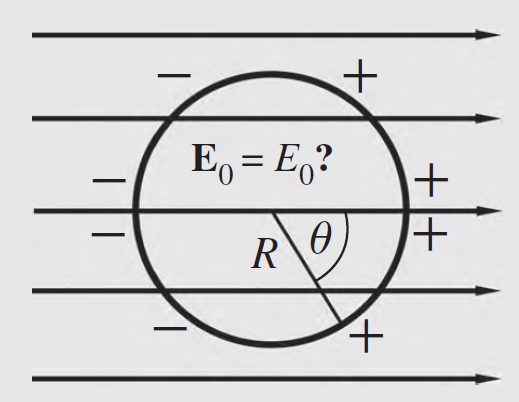
\includegraphics{2020/01/zangwill_fig_5_2.png}
    \caption{Zangwill Fig.~5.2.}
    \label{fig:zangwill_fig_5_2}
\end{figure}

Suppose now we have some strangely-shaped conductor with a cavity machined out of it, and we place a small (say, positive) charge inside the cavity. Well, what happens to the charge in the conductor? Clearly the inside surface of the cavity must rearrange itself to cancel the field within the conductor. That takes some net negative charge on the inside surface. That is, negative charge accumulates to shield the interior. That charge had to come from somewhere, though. There must be a net positive charge on the exterior surface which rearranges itself in some energetically favorable way. The neat thing is that the solution on the exterior surface doesn't depend at all on the shape of the cavity, or where the charge is placed inside. This is what we mean by shielding. Our conductor hides the details of the interior and reveals only the net charge contained within.
    
%week 3
%no lecture Tuesday due to MLK day
\section{Thursday, January 23, 2020}
    In full generality, we have an expression for the electrostatic potential near some charge distribution $\rho(\vec r)$:
\begin{equation}
    \varphi(\vec r)  =\frac{1}{4\pi \epsilon_0} \int d^3 r' \frac{\rho(\vec r')}{|\vec r- \vec r'|}.
\end{equation}
However, this denominator is complicated; it depends both on $\vec r'$, which we integrate over, and also $\vec r$, which we don't. A very nice way to decompose this expression is in terms of Legendre polynomials, as
\begin{equation}
    \frac{1}{|\vec r - \vec r'|} = \sum_{l=0}^\infty \frac{r'{}^l}{r^{l+1}} P_l(\uv r \cdot \uv r').
\end{equation}
If We're only interested in the potential on e.g. the $z$-axis, then this might be a good expansion to use. In that case, integrating over $\uv r'$ is not too bad. But if we're interested in more general $\vec r$ (say, ranging over a sphere), we still want to separate the angles, and we can instead use the angle addition formula for the spherical harmonics, which says
\begin{equation}
    \frac{1}{|\vec r - \vec r'|} = \sum_{l=0}^\infty \frac{r'{}^l}{r^{l+1}} \frac{4\pi}{2l+1} \sum_{m=-l}^l Y_{lm}(\theta, \phi) Y_{lm}^*(\theta',\phi').
\end{equation}

\subsection*{Capacitance}
Recall that the capacitance is defined as
\begin{equation}
    C= \frac{Q}{V},
\end{equation}
where $V$ is the potential relative to infinity. In a sense, the self-capacitance is the capacitance of the object with the other plate being a hollow sphere of infinite radius.

We're going to skip the details of the capacitance matrix and many-conductor systems; our main interest will be in systems with precisely two conductors, i.e. capacitors. Typically we put a $+Q$ charge on one and a $-Q$ charge on the other. These charges produce a potential difference $V$ between the conductors, such that the ratio $C=Q/V$ is the capacitance.

The prototypical example is the parallel-plate capacitor, with two plates of area $A$ and charge $+Q$ and $-Q$. So long as the plate separation $d$ is much less than the lateral dimension $\sqrt{A}$, i.e. $\sqrt{A} \gg d$, we can approximate these as infinite plates. It follows that
\begin{equation}
    \vec E = - \frac{Q}{\epsilon_0 A} \uv z, \quad V = -\int_0^d E\, dz = \frac{Qd}{\epsilon_0 A},
\end{equation}
so that
\begin{equation}
    C= \frac{Q}{V} = \frac{\epsilon_0 A}{d}.
\end{equation}
Let's note that our plates aren't really infinite, so the fringing effects at the edges mean that the $E$-field is weaker at the edges. It follows that the potential difference is lower for the same charge, so the capacitance goes up. Apparently we have \emph{underestimated} the capacitance.

Now we can calculate the energy in the capacitor as
\begin{equation}
    U=\frac{1}{2}\int d^3 r \rho(\vec r) V(\vec r)
\end{equation}
Notice that if we have two conductors, this integral simplifies considerably. Suppose we have one conductor with a surface $S_1$ and a charge $+Q$ and another conductor with a surface $S_2$ and a charge $-Q$. Conductors are equipotentials, and it follows that since all the charge lies on the surface, the integral becomes
\begin{equation}
    U= \frac{1}{2} \bkt{\int_{S_1} d^2 S \sigma_+(\vec r) V_+ + \int_{S_2} d^2S \sigma_-(\vec r) V_-} = \frac{1}{2} \bkt{V_+ Q + V_- (-Q)} = \frac{1}{2} QV,
\end{equation}
since $V=V_+ - V_-$ is the difference in the potentials. We can rewrite this as
\begin{equation}
    U= \frac{1}{2} \frac{Q^2}{C} = \frac{1}{2} CV^2,
\end{equation}
and this has interesting consequences depending on whether we hold charge constant or voltage constant. That is, if we hold charge constant, then it makes sense that a higher-capacitance (in the case of parallel plates, smaller $d$) setup is energetically favored. But if we hold voltage constant, then the plates actually want to push apart (lower capacitance).

For our parallel plate capacitor, we can check that this works by integrating the energy in the $E$-field:
\begin{equation}
    U_\parallel = \frac{1}{2} \epsilon_0 \int E^2 d^3r = \frac{\epsilon_0}{2} \frac{Q^2}{\epsilon_0^2 A^2} Ad = \frac{1}{2} QV.
\end{equation}

\begin{exm}[The quantum dot]
    We've just found that the self-energy of an object is given by
    \begin{equation}
        U= \frac{Q^2}{2C}.
    \end{equation}
    For objects with large self-capacitances, adding a bit of charge doesn't affect the total energy much. But for very small objects on the nanoscale, this self-capacitance can be very small, so it may take a lot of energy to change the charge by a little bit. That is, $U$ looks like a parabola centered at zero, and if we apply a ``gate voltage,'' we can shift the zero over to e.g. $Q=1/2$, so that whether we have $0$ or $1$ (electron) charges in the dot, both are equally favorable from an energy standpoint. Adding temperature into the picture can mess this up, though. Once the energy scale $k_BT$ becomes comparable to the energy cost of adding a charge, thermal effects will destroy this nice zero-or-one picture.
\end{exm}
%things will get worse before they get better

\subsection*{Dielectrics (Zangwill Ch. 6)}
Conductors are nice because their charge carriers redistribute to cancel applied electric fields. But insulators are more complicated because their cancellation is imperfect due to subtle material properties.

In materials, we can write the total charge $\rho$ as a sum of two terms-- a free (applied) charge and a polarization/bound charge due to the material response. That is,
\begin{equation}
    \rho(\vec r) = \rho_f(\vec r) + \rho_P(\vec r).
\end{equation}
The free charge $\rho_f$ is charge we control by putting it on objects, while the polarization (bound) charge $\rho_P$ is how the material responds to the applied charge/fields. For instance, in conductors, all the $\rho_P$ (i.e. the induced charge) lies on the surface of the conductor.

If we consider a dielectric with no net charge, then
\begin{equation}\label{eqn:unchargeddielectric}
    \int_V d^3 r\, \rho_P(\vec r) + \int_S d^2S \, \sigma_P(\vec r) =0.
\end{equation}
That is, the sum of the polarization volume charge and the polarization surface charge is zero.

We can then motivate the polarization vector $\vec P(\vec r)$ in the following way. A polarization vector should describe how charges redistribute in a material, such that
\begin{gather}
    \vec P(\vec r) = 0 \text{ outside the material},\\
    \vec P(\vec r) \cdot \uv n = \sigma_P(\vec r) \text{ on surface}.
\end{gather}
We can plug this into our equation~\eqref{eqn:unchargeddielectric} to get
\begin{equation}
    \int_V d^3 r\, \rho_P(\vec r) + \int_V d^3r\, \div \vec P(\vec r) =0
\end{equation}
by the divergence theorem. Since these are both volume integrals, it follows that the integrand vanishes,
\begin{equation}\label{eqn:divp}
    \div \vec P(\vec r) = -\rho_P(\vec r) \text{ inside material.}
\end{equation}

We can now integrate the polarization over the volume of the material. Note that $\grad_i r_j= \delta_{ij}$, so
\begin{equation}
    \int_V d^3 r\, P_j  = \int d^3r\, P_i \grad_i r_j = \int_V d^3r\, \grad_i(r_j P_i) - \int_V d^3r \, r_j \grad_i P_i
\end{equation}
by the chain rule. Then the first term is a divergence, so we can turn it into a surface integral, i.e.
\begin{equation}
    \int_V d^3r\, P_j = \int_S d^2 S\, r_j \sigma_P(\vec r) + \int_V d^3 r \, r_j \rho_P(\vec r)
\end{equation}
using the definitions of the polarization volume charge and surface charge. But now we recognize that these are moment integrals of charge distributions, which means that these are precisely in the form of a dipole moment. That is,
\begin{equation}
    \int_V d^3r \,\vec P = \vec p,
\end{equation}
the net dipole moment of the distribution. Hence we can think of polarization as dipole moment per unit volume.

Question: which quantity has more information, $\vec P(\vec r)$ or $\rho(\vec r)$? A priori, we might think that because of Eqn.~\eqref{eqn:divp}, the charge density has less information than the polarization vector, since we've taken a derivative (which is a lossy operation). But if we take the integral $\int_V d^3r \vec P = \vec p$, we only specify one moment of the distribution.

As it turns out, the polarization has more information because it contains phase information. That is, the integral tells us one piece of information we can extract from $\vec P$, but there's in principle more we can do with $\vec P$.
\end{document}